\documentclass{article}
% Pakker
\usepackage[utf8]{inputenc} % Så må vi bruge æ, ø og å
%\usepackage[ansinew]{inputenc}
%\usepackage[danish]{babel} % Dansk opsætning
\usepackage[T1]{fontenc} % Hjælper med ordeling ved æ, ø og å. Sætter fontene til at være ps-fonte i stedet for bmp.
\usepackage[english,final]{varioref} % Vi kan anvende \vref
\usepackage{array,booktabs} % Til gode tabeller
\usepackage{acronym} % Smart akronymhåndtering
\usepackage{minitoc} % Vi kan lave del inholdsfortegnelser forhåbentlig
\usepackage{bytefield}
\usepackage{epsfig}
\usepackage{amsmath}
\usepackage{mathtools}
\begin{document}
\chapter{Modelling}
\section{List of acronyms}
\begin{acronym}[TDMA]
  \acro{SSS}{Single Screw Ship}
  \acro{TSS}{Twin Screw Ship}
  \acro{IMU}{Inertial Measurement Unit}
\end{acronym}

\section{Modelling of Twin Screw Ship}
When modelling the forces affecting a \ac{TSS} there few parameters which affect the movement of the ship. These are the forces applied by the motors, as well as the placement of the motors. For calculating these contributions simple trigonometric functions can be used. This gives the resulting forces in the boats X and Y directions, as well as the torque generated.
\begin{figure}
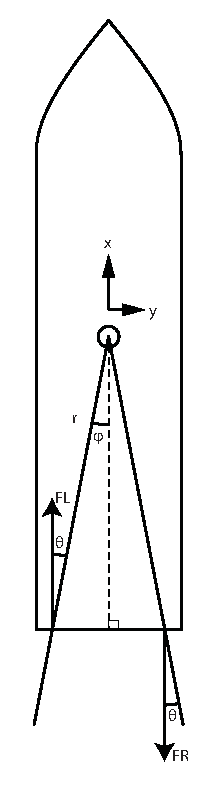
\includegraphics{img/boatmodel.pdf}[h]
\caption{By controlling FL and FR, it is possible to control the translational and rotational forces of the ship. The division of these forces is dependant on the angle of attack, $\theta$.}
\end{figure}
First we see that the boat is mirrored along it's X axis. From this we can set $\theta = \theta_L = \theta_R$ and $\phi = \phi_L = \phi_R$.  Now we have the forces, $F_L$ and $F_R$, as the controllable input to our system. These will be divided as into $F_X$, $F_Y$ and $\tau$, which are the variables that we wish to control. This division takes the form as seen in equation \eqref{Forceequation}.

\begin{equation}
\left[
\begin{matrix}
F_x\\
F_y\\
\tau
\end{matrix}
\right]
 =
 \left[
\begin{matrix}
cos(\phi - \theta)\\
sin(\phi - \theta)\\
sin(\theta) \cdot r
\end{matrix}
\right]
\cdot F_R
+
 \left[
\begin{matrix}
cos(\phi - \theta)\\
sin(\phi - \theta)\\
-sin(\theta) \cdot r
\end{matrix}
\right]
\cdot
F_L
\label{Forceequation}
\end{equation}
We observe that the motors will deliver force parallel to the x-axis, we can further set $\theta = \phi$. If this is the case $sin(\theta - \phi)=0$, which nullifies the $F_Y$ term, and $cos(\theta-\phi) = 1 \Longrightarrow F_X = F_L+F_R$ . The forces can then be modelled as equation \eqref{shortformforces}.
\begin{equation}
\left[\begin{matrix}
F_X\\
\tau
\end{matrix}
\right]
= 
\left[
\begin{matrix}
1\\
sin(\theta)\cdot r
\end{matrix}
\right]
\cdot F_R
+ 
\left[
\begin{matrix}
1\\
-sin(\theta)\cdot r
\end{matrix}
\right]
\cdot F_L
\label{shortformforces}
\end{equation}

\section{State Space form}
For better control of the system, it is desired to have the model of the ship in State Space form. This makes it possible to design an observer and a controller, which further makes it possible to design poles and zeros of the system.

The state space form for the system has the general form 
\begin{figure}[h]

\begin{equation}
\dot{x}=Ax+Bu
\end{equation}
\begin{equation}
y=Cx+Du
\end{equation}
\begin{tabbing}
Where \= $x$ is the state vector.\\
	\> $\dot{x}$ is the derivative of the state vector.\\
	\> $A$ is the state matrix\\
	\> $B$ is the input matrix\\
	\> $y$ is the output vector\\
	\> $C$ is the output matrix\\
	\> $D$ is the feedforward matrix
	
	
\end{tabbing}
\end{figure}
\end{document}